\begin{song}{title=\predtitle\centering Je jaká je \\\large Karel Gott  \vspace*{-0.3cm}}  %% sem se napíše jméno songu a autor
\begin{centerjustified}
\nejnejvetsi

\sloka
Je, ^{D\z}jaká ^{F#mi G}je, tak mi ^*{A}ná hle padla ^{D}do ^{\z F#mi}klína,~~~~~~

^{G\z}~~ani ^{A\z}černá ani ^{D\z F#mi G}blondýna,~~~~~ někdy ^{A}tak a jindy ^{D{\color{white}\_\_}}taková, ^{Hmi}

^{G\z}~~vždycky ^{A\z}hádám, jak se ^{D\z Hmi G}zachová,~~~~~ zřejmě ^{A\z}nikdy, jak chci ^{D}já.

^{Hmi G A}

\sloka 
Je, jaká je -- trochu dítě, trochu mondéna,

nemám právě paměť na jména, tak jí říkám lásko má.

Nejsi skvost a nejsi zlá, jsi jen jiná, než chci já.

\sloka
Je, jaká je, že se změní čekat nedá se,

snad jí záleží jen na kráse, tak, že člověk málem nedutá,

jak je štíhlá, jak je klenutá, jenže jinak, než chci já.

\sloka
Je, jaká je, až ji zitra spatříš u pláže,

vzkaž jí, ať se na mě neváže, ať si pro mě vrásky nedělá,

ať je jaká je a veselá, i když jiná, než chci já.

\end{centerjustified}
\setcounter{Slokočet}{0}
\end{song}


\begin{figure}[h]
\predtitle\centering
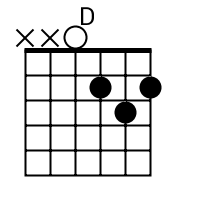
\includegraphics[width=3cm]{../Akordy/d.png}
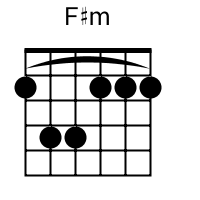
\includegraphics[width=3cm]{../Akordy/fxm.png}
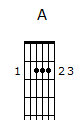
\includegraphics[width=3cm]{../Akordy/a.png}
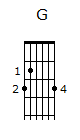
\includegraphics[width=3cm]{../Akordy/g.png}
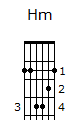
\includegraphics[width=3cm]{../Akordy/hm.png}
\end{figure}
